\section{Memory}

The memory hierarchy is one of the more complicated concepts in MMIX. This section starts by explaining the load and store instructions, which are rather simple. Afterwards the structure of the virtual and physical address space is described, followed by the translation mechanism and the translation caches. Finally, the instructions interesting for physical memory caches, which may be present in a particular implementation of MMIX, are introduced.

\subsection{Load Instructions}

MMIX has two kinds of load instructions for each quantity: a signed version and an unsigned version. The difference is that the signed versions treat the number in memory as signed and thus sign-extend the value to 64 bit.

\instrtbl
	{\mi{LDB|LDW|LDT|LDO \$X,\$Y,\$Z|Z}}
	{$\dr{X} \leftarrow s(\vmem{1|2|4|8}{\dr{Y} + \udrim{Z}})$}
\noindent These are the signed load instructions, which set \dr{X} to the byte, wyde, tetra or octa at the specified location in memory. \mi{LDB}, \mi{LDW} and \mi{LDT} will sign-extend the number, \ie the bits in the upper 7, 6 and 4 bytes, respectively, are set to copies of the sign-bit of the number in memory. \citep[pg. 4]{mmix-doc}

\instrtbl
	{\mi{LDBU|LDWU|LDTU|LDOU \$X,\$Y,\$Z|Z}}
	{$\dr{X} \leftarrow $~\vmem{1|2|4|8}{\dr{Y} + \udrim{Z}}}
\noindent As already mentioned, the unsigned versions have the same behaviour, except that they do not sign-extend the values. \mi{LDOU} and \mi{LDO} are completely identical and only exist both for consistency. \citep[pg. 4]{mmix-doc}

\instrtbl
	{\mi{LDHT \$X,\$Y,\$Z|Z}}
	{$\dr{X} \leftarrow~\vmem{4}{\dr{Y} + \udrim{Z}}~\ll 32$}
\noindent The last load instruction, \i{load high tetra}, puts the tetra \vmem{4}{\dr{Y} + \udrim{Z}} into the higher half or \dr{X}. The other half is set to zero. \citep[pg. 4]{mmix-doc}

\subsection{Store Instructions}

Analogous to the load instructions, MMIX provides two store instructions for every quantity. In this case, the signed versions throw an integer overflow \glslink{Exception}{AE}, if the number can not be represented with the corresponding quantity, while the unsigned versions do not.

\instrtbl
	{\mi{STB|STW|STT|STO \$X,\$Y,\$Z|Z}}
	{$\vmem{1|2|4|8}{\dr{Y} + \udrim{Z}}~\leftarrow s(\dr{X})$}
\noindent These instructions write the signed number in \dr{X} to the corresponding location in memory. \mi{STB} will throw an integer overflow \glslink{Exception}{AE}, if \dr{X} is not between $-128$ and $+127$, \mi{STW} if \dr{X} is not between $-32,768$ and $+32,767$ and \mi{STT} if \dr{X} is not between $-2,147,483,648$ and $+2,147,483,647$. \mi{STO} will not throw an integer overflow \glslink{Exception}{AE}. \citep[pg. 5]{mmix-doc}

\instrtbl
	{\mi{STBU|STWU|STTU|STOU \$X,\$Y,\$Z|Z}}
	{$\vmem{1|2|4|8}{\dr{Y} + \udrim{Z}}~\leftarrow \dr{X}$}
\noindent The unsigned store instructions are the same as their signed correspondence, but do not test for overflow. \citep[pg. 5]{mmix-doc}

\instrtbl
	{\mi{STHT \$X,\$Y,\$Z|Z}}
	{$\vmem{4}{\dr{Y} + \udrim{Z}}~\leftarrow \dr{X} \gg 32$}
\noindent Similarly to load high tetra, \i{store high tetra} stores the most significant four bytes of \dr{X} to \vmem{4}{\dr{Y} + \udrim{Z}}. \citep[pg. 5]{mmix-doc}

\instrtbl
	{\mi{STCO X,\$Y,\$Z|Z}}
	{$\vmem{8}{\dr{Y} + \udrim{Z}}~\leftarrow {\tt X}$}
\noindent For convenience and efficiency, MMIX provides another store instruction, \i{store constant octabyte}, which stores the unsigned \glslink{Immediate Value}{immediate value} {\tt X} as an octa to the desired location in memory. This saves the programmer from having to put the constant into a register first. \citep[pg. 5]{mmix-doc}

\subsection{Virtual and Physical Address Space}

As already mentioned at the beginning, MMIX has both a 64-bit virtual and physical address space. Their layout is illustrated by the following figure:
\begin{figure}[H]
	\centering
	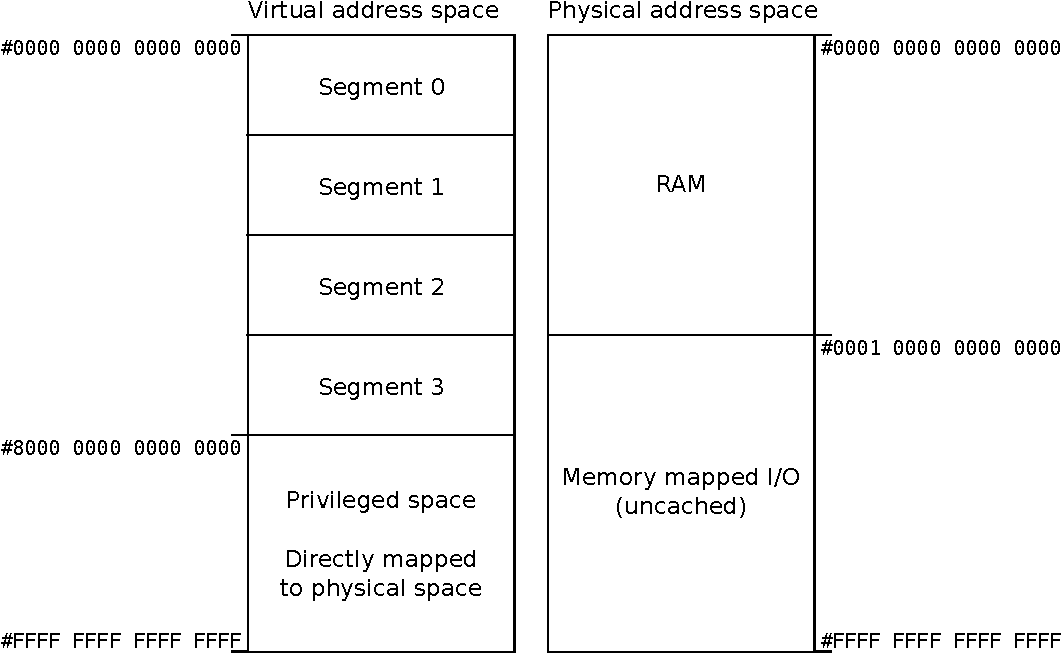
\includegraphics[width=\textwidth]{img/address-spaces-crop.pdf}
	\caption{Virtual and physical address space layout \citep[pg. 35]{mmix-doc}}
\end{figure}
\noindent The virtual address space is divided in user space and privileged space. The privileged space is directly mapped to the physical address space, called m. That means, \vmem{}{{\tt X}}$~=~$m[${\tt X}~\land~$\haddro{7FFF}{FFFF}{FFFF}{FFFF}$]$, if ${\tt X} \ge 2^{63}$. The user space is divided into four segments, determined by the most significant 3 bits using $000_2$, $001_2$, $010_2$ and $011_2$ for segment 0, 1, 2 and 3, respectively. The use of these segments is not restricted by the hardware, but each segment is translated separately, as will be described in the next section.

The first 256 terabyte of the physical space are used for RAM. The remaining space is reserved for I/O devices. The layout of the I/O space is implementation dependent, but MMIX defines that the I/O space is always uncached, regardless of whether the particular MMIX implementation uses caching or not. \citep[pg. 35]{mmix-doc}

\subsubsection{Address Translation}

Besides the privileged space, which is directly mapped to the physical space, the user space is translated to the physical one via a quite complicated scheme. This section describes how this translation works in detail.

\paragraph{The Virtual Translation Register}

The translation is defined by register \sr{V}, which has the following layout:
\begin{figure}[H]
	\centering
	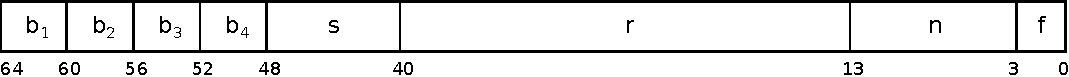
\includegraphics[width=\textwidth]{img/rV-crop.pdf}
\end{figure}
\vspace{-20pt}
\noindent The first two bytes of \sr{V} specify the number of pages in the four segments. Segment $i$ has at most $1024^{b_{i+1}-b_i}$ pages, where $b_0$ is defined to be zero. If $b_i = b_{i+1}$, segment $i$ must have at most one page and if $b_i > b_{i+1}$, segment i must be empty. For example,
\begin{itemize}
	\item if $b_1 = 1$, $b_2 = 2$, $b_3 = 3$ and $b_4 = 4$, all segments will have at most 1024 pages,
	\item if $b_1 = 3$, $b_2 = 2$, $b_3 = 1$ and $b_4 = 0$, segment 0 will have at most $1024^3$ pages and all other segments will be empty and
	\item if $b_1 = 1$, $b_2 = 0$, $b_3 = 0$ and $b_4 = 0$, segment 0 will have at most 1024 pages, segment 1 will be empty and segments 2 and 3 will have both at most 1 page.
\end{itemize}
The next field, called $s$, specifies that the page size is $2^s$, where $s$ has to be at least 13 and at most 48. The field $r$ tells MMIX the \i{root location}, which will be described in further detail shortly. The field $n$ holds the \i{address space number} and last but not least, $f$ is the \i{function field}, which specifies whether virtual address translation will be done by software ($f=1$) or by hardware ($f=0$). Other values are illegal. If translation by software is requested, MMIX will ignore $b_1$, $b_2$, $b_3$, $b_4$ and $r$ of \sr{V} and let the software decide how the actual translation mechanism works. That means, the following structures and concepts only apply if hardware translation is used. \citep[pg. 36]{mmix-doc}

\paragraph{The Root Location}

The field $r$ specifies an area in memory that holds the \glslink{Paging}{paging} structures for the current virtual address space. For each segment $i$ it holds $b_{i+1} - b_i$ page tables with either \i{page table entries} (PTEs) or \i{page table pointers} (PTPs), which are described in the next paragraphs. The page tables in the root location are, one could say, the "first layer" of the translation, because PTPs point to other page tables that reside in a different location in memory.

\paragraph{Page Table Entries}

A PTE defines to which page in physical memory a page in virtual memory is mapped to. Additionally it specifies the access permissions for that page. A PTE looks like the following:
\begin{figure}[H]
	\centering
	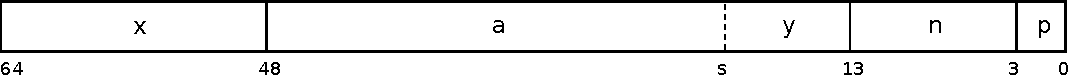
\includegraphics[width=\textwidth]{img/PTE-crop.pdf}
\end{figure}
\vspace{-20pt}
\noindent The field $a$ holds the physical address divided by the page size, \ie the physical address is $a * 2^s$. The field $n$ is the address space number, which has to be equal to $n$ in \sr{V}. The access permissions are defined by $p$ with bit 0 for executing, bit 1 for writing and bit 2 for reading. That means, for example $p=101_2$ makes the page readable and executable. The fields $x$ and $y$ are ignored by the hardware, which allows the operating system to use them for any purpose. \citep[pg. 36]{mmix-doc} It is noteworthy, that $y$ would be empty, if the page size were $2^{13}$, and $a$ would be empty, if the page size were $2^{48}$. Additionally, the layout of a PTE clarifies the reason for the page size restrictions.

\paragraph{Page Table Pointers}

PTPs are pointers to other page tables that may either hold PTPs as well or hold PTEs. They have the following layout:
\begin{figure}[H]
	\centering
	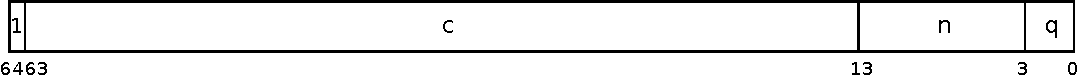
\includegraphics[width=\textwidth]{img/PTP-crop.pdf}
\end{figure}
\vspace{-20pt}
\noindent Similarly to the field $a$ of a PTE, the field $c$ of a PTP specifies the address of the page table this PTP links to, divided by the page size. The field $n$ has to match $n$ in \sr{V} as well, while $q$ is ignored and the most significant bit has to be 1. This forces the operating system to put a privileged address into a PTP, which is -- as already mentioned -- directly mapped. \citep[pg. 36]{mmix-doc}

\paragraph{The Translation Process}

Finally, the actual translation process should be described. If address $A$ should be translated, the segment is determined by $i = \lfloor A / 2^{61} \rfloor$. The page number in this segment is $A_p = \lfloor (A~\land~$\haddro{1FFF}{FFFF}{FFFF}{FFFF}$) / 2^s \rfloor$. Assuming that $A_p$ is equal to $(a_4a_3a_2a_1a_0)_{1024}$ (in the number system with base 1024), the translation works as follows:
\begin{itemize}
	\item if $a_4=a_3=a_2=a_1=0$, the PTE $e$ is \pmem{8}{2^{13}(r + b_i) + 8a_0} and thus, \vmem{}{A} corresponds to \pmem{}{2^s*e.a + (A \bmod 2^s)}.
	\item if $a_4=a_3=a_2=0$, the auxiliary PTP $p$ is used, \ie \pmem{8}{2^{13}(r + b_i + 1)+8a_1}. In this case, the PTE is \pmem{8}{2^{13}*p.c + 8a_0}. Thus, one level of indirection is involved.
	\item if $a_4=a_3=0$, two levels of indirection are used. That means, the first PTP $p1$ is \pmem{8}{2^{13}(r + b_i + 2)+8a_2} and determines the next PTP. This one, $p2$, is \pmem{8}{2^{13}*p1.c + 8a_1}. And finally the PTE is \pmem{8}{2^{13}*p2.c + 8a_0}.
	\item \dots
\end{itemize}
\citep[pg. 36]{mmix-doc} It is noteworthy, that when using the minimum page size of $2^{13}$, four levels of indirection are sufficient to cover a whole segment. Because $2^{13} * 1024 * 1024^4 = 2^{63}$ covers even more than one segment. Additionally, it is worth mentioning that the first slot in PTP page tables in the root location is actually never used. Because this slot is covered by the previous page table in the root location.

\paragraph{Example}

To clarify the just explained concepts and to show the layout in memory, which they imply, the following goes through an example. Supposed that \sr{V} and the \glslink{Paging}{paging} structures in memory are filled as:
\begin{figure}[H]
	\centering
	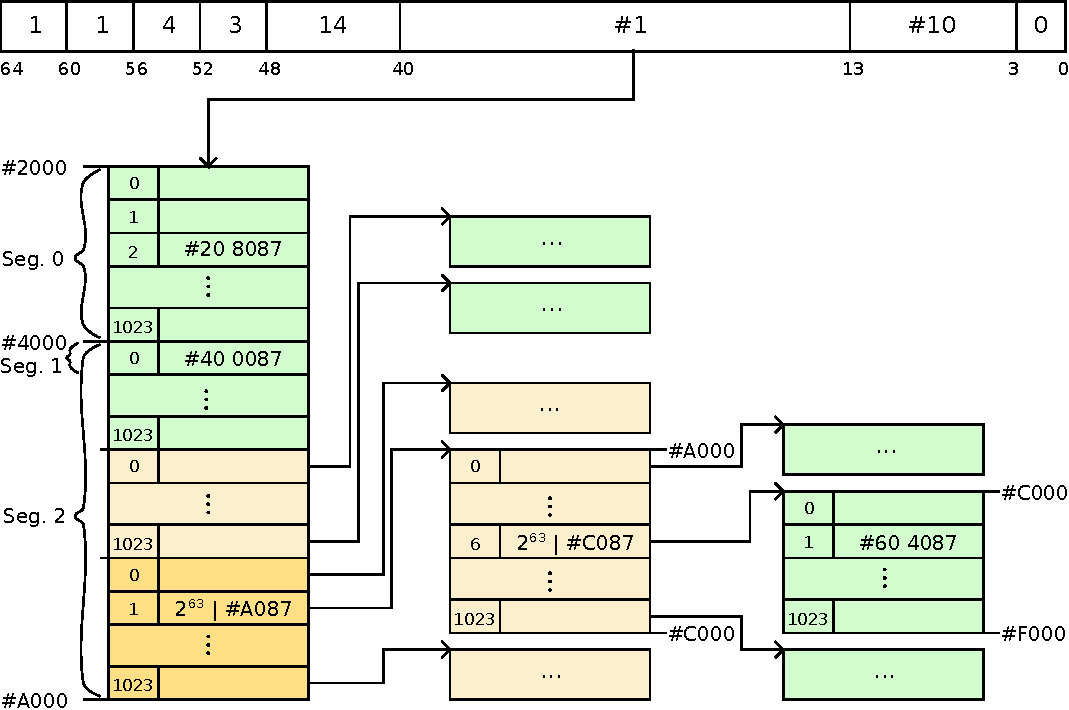
\includegraphics[width=\textwidth]{img/paging-example-crop.pdf}
	\caption{Paging example}
\end{figure}
\noindent Hence, segment 0 has 1024 pages, segment 1 has only one page, segment 2 has $1024^3$ pages and segment 3 has no pages at all. Additionally, the page size is $2^{14}$, the address space number is \haddr{10} and the root location is \haddr{2000} (\haddr{1}$~\ll 13$). The root location is displayed on the left, while auxiliary page tables are on the right. Furthermore, the green cells contain PTEs, the light orange cells PTPs of level 1 and the orange cells PTPs of level 2. For demonstration purposes, the cells display the page table index on the left and some show the content as an octa on the right. All PTEs and PTPs end with \haddr{87}, because they have to match the $n$ of \sr{V} and have read, write and execute permissions (which actually has no special reason here).

Ignoring the special case that segment 1 and 2 overlap for a while, one can see that the number of page tables in the root location for segment $i$ corresponds to $b_{i+1} - b_i$. The first page table does always contain PTEs, the second one PTPs of level 1 and so on. Each page table has 1024 slots and therefore it is 8192 bytes large. As the arrows show, PTPs do always point to another page table.

Since in this case $b_1$ is equal to $b_2$, segment 1 has only one page. An additional consequence of the interpretation of the segment sizes and the translation mechanism is, that -- as the figure shows -- the page in segment 1 is mapped by the first PTE of the page table responsible for segment 2. Thus, this PTE is used for the first page both in segment 1 and segment 2.

To demonstrate the translation process, the following shows a few examples:
\begin{itemize}
	\item Virtual address \haddr{80FF}:\\
	Obviously, \haddr{80FF} belongs to segment 0 and the page number is $(00002)_{1024}$. As described, in this case the PTE is \pmem{8}{2^{13}($\lstinline`\#1`$+0) + 8*2}$~=~$\pmemh{8}{2010}. The third slot of the first page table in segment 0 contains \haddrt{20}{8087}, which means that the physical base address for that page is \haddrt{20}{8000} and thus, the resulting physical address \haddrt{20}{80FF}.
	\item Virtual address \haddro{2000}{0000}{0000}{1234}:\\
	This address belongs to segment 1 and has the page number $(00000)_{1024}$. The PTE is \pmem{8}{2^{13}($\lstinline`\#1`$+1) + 8*0}$~=~$\pmem{8}{$\lstinline`\#4000`$}$~=~$\haddrt{40}{0087}. Hence, the resulting physical address is \haddrt{40}{1234}.
	\item Virtual address \haddro{4000}{0004}{0600}{4000}:\\
	Last but not least, this address belongs to segment 2 and has the page number $(00161)_{1024}$. Thus, the level 2 PTP is \pmem{8}{2^{13}($\lstinline`\#1`$+3) + 8*1}$~=~$\pmemh{8}{8008}, which loads \haddro{8000}{0000}{0000}{A087}. Therefore it links to the PTP \pmem{8}{$\lstinline`\#A000`$ + 8*6}, \ie \pmemh{8}{A030}, which in turn is \haddro{8000}{0000}{0000}{C087}. The last step loads the PTE \pmem{8}{$\lstinline`\#C000`$ + 8*1} $=~$\pmemh{8}{C008}$~=~$\haddrt{60}{4087}, so that the final address is \haddrt{60}{4000}.
\end{itemize}

\subsubsection{Translation Caches}

To prevent that every memory access requires this lengthy translation from virtual to physical addresses, MMIX uses a \i{translation cache}. This is also known as \i{translation lookaside buffer} (TLB). However, MMIX calls it translation cache or short TC. The exact behaviour or whether separate caches for instructions and data exist, is not enforced by the architecture. But MMIX defines that the TC contains \i{translation keys}, which are associated with \i{translations}. The translation key is basically the virtual address, whereas the translation is more or less the physical address. The key is structured as follows:
\begin{figure}[H]
	\centering
	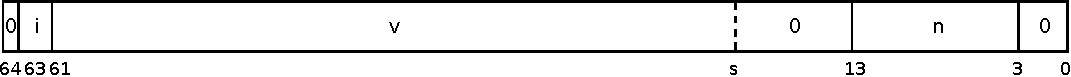
\includegraphics[width=\textwidth]{img/TC-key-crop.pdf}
\end{figure}
\vspace{-20pt}
\noindent As usual, the field $n$ holds the address space number. The field $i$ is the segment number and $v$ is the virtual address in that segment, divided by the page size. The other parts are defined to be zero. The layout of a translation is:
\begin{figure}[H]
	\centering
	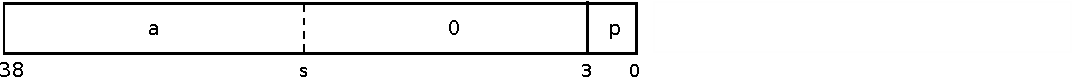
\includegraphics[width=\textwidth]{img/TC-trans-crop.pdf}
\end{figure}
\vspace{-20pt}
\noindent Similarly to a PTE, the field $a$ holds the physical address, divided by the page size. The last three bits contain the protection bits, whereas the other bits are defined to be zero. \citep[pg. 37]{mmix-doc}

Of course, the operating system needs a way to keep the TC up to date, when for example removing PTEs or changing their protection bits. Therefore, MMIX provides the instruction \mi{LDVTS}.

\instrtbl
	{\mi{LDVTS \$X,\$Y,\$Z|Z}}
	{$\dr{X} \leftarrow updateTC(\dr{Y} + \udrim{Z})$}
\noindent The instruction \i{load virtual translation status} updates the translation cache for $\dr{Y} + \udrim{Z}$, which should have the form of a translation key, except that the least significant three bits need not be zero. \dr{X} will be set to 0 if the key is not in the TC, 1 if it is present for instructions, 2 if it is present for data and 3 if it is present for both. If this key is present in the TC, the protection bits will be replaced with $(\dr{Y} + \udrim{Z})~\land~$\haddr{7}. If these are zero, the key will be removed. \citep[pg. 37]{mmix-doc}

\subsubsection{Physical Memory Caches}

As already mentioned, a particular implementation of MMIX may use caches for the RAM space of the physical memory. Which caches are present and how they are organized, is completely implementation dependent. But MMIX provides several instructions to allow a more efficient use of the caches and to keep them up to date. Similarly to the translation caches, MMIX has in mind that an implementation may provide separate caches for instructions and data.

\instrtbl
	{\mi{LDUNC \$X,\$Y,\$Z|Z}}
	{$\dr{X} \leftarrow s(\vmem{8}{\dr{Y} + \udrim{Z}})$}
\noindent The first instruction in this category is \mi{LDUNC}, \i{load octa uncached}. It has  the same behaviour as \mi{LDO}, but tells MMIX "that the loaded octabyte (and its neighbors in a cache block) will probably not be read or written in the near future" \citep[pg. 24]{mmix-doc}.

\instrtbl
	{\mi{STUNC \$X,\$Y,\$Z|Z}}
	{$\vmem{8}{\dr{Y} + \udrim{Z}}~\leftarrow s(\dr{X})$}
\noindent The instruction \i{store octa uncached} has the same meaning as \mi{STO} and tells MMIX the same as \mi{LDUNC} does. \citep[pg. 24]{mmix-doc}

\instrtbl
	{\mi{PRELD|PREGO|PREST X,\$Y,\$Z|Z}}
	{-}
\noindent These instructions have no (visible) effect, but inform MMIX that the ${\tt X}+1$ bytes \vmem{1}{\dr{Y} + \udrim{Z}}, \dots, \vmem{1}{\dr{Y} + \udrim{Z} + {\tt X}} will probably be loaded/stored, used as instructions or stored before loaded for \mi{PRELD}, \mi{PREGO} or \mi{PREST}, respectively. That means, if \mi{PRELD} is used, it might make sense to load these bytes into the data cache. If \mi{PREGO} is used, MMIX might put these bytes into the instruction cache and if \mi{PREST} is used, MMIX may ignore the current bytes in memory. Therefore, if these bytes are requested and are not yet in cache, MMIX does not need to load them from memory, because they will be written before they are read anyway. MMIX does also define, that no protection fault occurs for these instructions. \citep[pg. 24]{mmix-doc}

\instrtbltwo
	{\mi{SYNCD X,\$Y,\$Z|Z}}
	{$caches[\dr{Y} + \udrim{Z}:{\tt X}+1] \rightarrow$~\pmem{}{\dr{Y} + \udrim{Z}:{\tt X}+1}}
	{if in privileged mode: $caches[\dr{Y} + \udrim{Z}:{\tt X}+1] \leftarrow \varnothing$}
\noindent The instruction \i{synchronize data} forces the hardware to make sure that all data for the ${\tt X}+1$ bytes \vmem{1}{\dr{Y} + \udrim{Z}}, \dots, \vmem{1}{\dr{Y} + \udrim{Z} + {\tt X}} is present in memory (and not only in cache). If executed in the privileged space, it does additionally force MMIX to remove these bytes from the data cache. Again, no protection fault will occur if the memory is not accessible. \citep[pg. 24]{mmix-doc}

\instrtblfour
	{\mi{SYNCID X,\$Y,\$Z|Z}}
	{if in user mode:}
	{$\quad IC[\dr{Y} + \udrim{Z}:{\tt X}+1] \leftrightarrow DC[\dr{Y} + \udrim{Z}:{\tt X}+1]$}
	{else:}
	{$\quad caches[\dr{Y} + \udrim{Z}:{\tt X}+1] \leftarrow \varnothing$}
\noindent When executed in user space, \i{synchronize instructions and data} forces the hardware to make sure that the ${\tt X}+1$ bytes \vmem{1}{\dr{Y} + \udrim{Z}}, \dots, \vmem{1}{\dr{Y} + \udrim{Z} + {\tt X}} will be interpreted correctly when used as instructions. That means, MMIX should synchronize its data cache with its instruction cache (\eg because instructions might have been manually fabricated and might thus only be present in the data cache yet). When \mi{SYNCID} is executed in privileged space, the hardware has to remove these bytes from all caches \i{without} writing it to memory. As with \mi{SYNCD}, no protection faults can occur. \citep[pg. 24,25]{mmix-doc}

\instrtbleight
	{\mi{SYNC XYZ}}
	{if ${\tt XYZ} = 0$: drain pipeline}
	{if ${\tt XYZ} = 1$: drain stores}
	{if ${\tt XYZ} = 2$: drain loads}
	{if ${\tt XYZ} = 3$: drain loads and stores}
	{if ${\tt XYZ} = 4$: go into power-saver mode}
	{if ${\tt XYZ} = 5$: flush caches to memory}
	{if ${\tt XYZ} = 6$: clear TCs}
	{if ${\tt XYZ} = 7$: clear caches}
\noindent The last instruction in this category is \i{synchronize}, which is used for various purposes, whereas the 24-bit constant {\tt XYZ} determines what action is performed. The first four actions drain the pipeline, in the sense that it stalls until all preceding instructions are finished (or all stores, loads, loads and stores for 1, 2, 3, respectively, are finished before the corresponding instructions after them). The fifth action tells MMIX to go into a power-saver mode, \ie MMIX is allowed to execute instructions slower or not at all until some kind of signal arrives. The next one writes all cache content to main memory, while the last two simply remove all entries from the TCs or the instruction and data caches. Using \mi{SYNC} with ${\tt XYZ} > 3$ is allowed in privileged mode only. \citep[pg. 25]{mmix-doc}

